\documentclass[english]{article}
\usepackage{graphicx} % Required for inserting images
\usepackage{hyperref}
\usepackage{url}
\usepackage[backend=bibtex8]{biblatex}
\addbibresource{references.bib}
\renewcommand\refname{}
\renewcommand*{\contentsname}{}
\graphicspath{{images}}

\title{Enhancing Network Intrusion Detection Robustness via Dataset Augmentation: A CIC-IDS-2017 Case Study
}
\author{Jozef Jankaj}
\date{May 2025}


\begin{document}
	
\maketitle

\tableofcontents
	
	\newpage
	
	\section{Introduction}
	A lot of time has passed since that fateful night of October 29, 1969, when the first inter-network communication took place through the ARPANET link. In his statement in an interview with Gregory Gromov
	
	\begin{center} 
		"Then we typed the G, and the system crashed… Yet a revolution had begun” \cite{kleinrock}
	\end{center}
	
	who knows if prof. Leonard Kleinrock had fully realized just how massive the revolution was going to be. 
	Since then, the internet has grown exponentially: from a small group of four nodes, through the invention of the World Wide Web by Sir Tim Bernes-Lee for the sharing of academic knowledge, via the dot-com bubble of the 2000's, to an inseparable part of our lives. As our lives have moved into cyberspace, so have threats against our privacy. We no longer face only the criminals on the streets, but also a threat from cybercriminals on the other side of the world. As such, protection measures have been developed, chief among which are Network Intrusion Detection Systems (NIDS). These systems monitor traffic within the network and send out alerts when malicious traffic is encountered, or even cut the connection altogether. 
	
	In recent years, NIDS research has explored how the capabilities of machine learning methods can be utilized to protect our networks. While many papers claim excellent performance and groundbreaking contributions, the field of machine learning-based NIDS (ML-NIDS) has been met with skepticism by practitioners \cite{sok_nids_assessment}, chief among them being the lack of evidence of generalization to different networks.
	
	The aim of this work is to address this complaint by verifying a method of enhancing robustness of NIDS datasets through dataset augmentation. As a point of study, we take the CIC-2017 dataset \cite{cic_2017} created by the Canadian Institute for Cybersecurity. 
	
	This work is structured as follows: In Section 2, we explore the literature surrounding ML-NIDS, illustrating current methods and datasets used in the field. In Section 3, we formulate a hypothesis behind the poor generalization performance of ML-NIDS models, explore the CIC-2017 dataset in-depth and recreate it using ConCap \cite{concap}. In Section 4, we present results of our testing. Finally, in Section 5, we draw conclusions and reflect on future work.
	
	\newpage
	\section{Literature study}\label{lit_study}
The problem NIDS systems solve inherently belongs to the category of classification problems: determine whether a particular network traffic is benign or malicious.

One of the first implementations of a Network Intrusion Detection System (NIDS) has been NADIR (Network Anomaly Detection and Intrusion Reporter) \cite{nadir} from 1990. This system was developed for the Integrated Computing Network at Los Alamos National Laboratory to automate the detection of unauthorized access to the system. NADIR utilized statistical profiles of network users to detect anomalies, notifying and printing out abnormalities in the profiles as detected by manually designed expert rules.

NADIR is an example of what we call "expert-made NIDS": it follows a strict set of rules to detect and report unauthorized activity, programmed by an expert. While these systems work well as first lines of defense, they also suffer from a fundamental flaw: they can only detect what they were specifically programmed to detect by their creators. This is a difficult task: given the sheer amount of information going through the network at any particular time, one does not (or can not) know which pieces of data point to malicious traffic. Furthermore, malicious packets in one context may be harmless in another or contents may be completely encrypted, further reducing the ability of humans to tell benign traffic apart from malicious. 

Instead of having to manually preprogram the NIDS with attack profiles, machine learning (ML) allows us to teach a model the distinction between malicious and benign traffic, by observing examples, leading directly to the concept of ML-NIDS: Machine Learning-based Network Intrusion Detection System.

In general, ML-NIDS can be split into two subgroups: signature-based and anomaly-based. Both subgroups fulfill the same task (tell malicious and benign traffic apart), but approach it in fundamentally opposite ways. Signature-based ML-NIDS is trained to recognise an attack, or even the specific kind of attack in multi-class classification: the "positive" label is the malicious traffic. On the contrary, anomaly-based ML-NIDS learns to recognise what benign traffic looks like, and triggers and alarm at any traffic that is "out of the ordinary". 

\newpage
\subsection{Machine Learning methods}
Machine-learning methods are a class of algorithms that have the computer infer relations and rules of a dataset by being exposed to training samples. As our focus is network intrusion detection, we focus on methods that perform classification: determination whether a particular sample is malicious or benign. These methods can generally be subdivided into two categories: Shallow Learning and Deep Learning. 

\subsubsection{Shallow Learning}
Some of the most widely known and used machine learning algorithms are:
\begin{enumerate}
    \item K-Nearest Neighbours (KNN) \cite{knn}: Initially developed by Fix and Hodges in 1951 \cite{fix_hodges} and later improved by Cover and Hart in 1967 \cite{knn}, these models can be used for multiclass classification. Predictions are formed by a majority vote, where the prediction is formed by the label of samples most similar to the input.
    \item Support Vector Machines (SVM) \cite{svm}: SVMs, originally developed by Cortes and Vapnik in 1995, are models used for binary classification. The model learns to distinguish between two labels by transforming inputs into a high-dimensional space. In this "feature" space, a hyperplane can be constructed to distinguish between the two labels. The binary classification can be extended into n-label classification by training a separate SVM (target label vs anything else) for each label and perform classification by having each SVM predict the label, with a unique SVM predicting its assigned label instead of "anything else".
    \item Decision Trees (DT) \cite{decision_trees}: Decision trees form a tree data structure, with each internal node testing for a particular feature in the data, reaching a class label in one of the leaf nodes.
    \item Ensemble methods \cite{ensemble}: Ensemble methods combine multiple simpler classifiers to form a larger one. This way, weaknesses of the underlying classifier (e.g. an SVM being unable to separate multiple classes) can be overcome (a separate SVM being trained for each class label, as described above).
\end{enumerate}

Liao and Vemuri \cite{knn_2002} use a KNN classifier for intrusion detection by building a profile of the input process consisting of the occurrences of system calls the process performs.

Sahu and Mehtre \cite{j48_dt} implement the J48 Decision Tree, testing it on Kyoto 2006+ dataset \cite{kyoto}. Their trained model boasts 97.23\% accuracy and a true positive rate of 99\% for normal and attack packets.  

Bao, Xu and Hou \cite{nids_svm} build an NIDS system consisting of two SVM models: one for anomaly detection, the other for misuse detection using previously seen attack signatures. Authors do make claims about "high training rate and decision rate, insensitiveness to dimensions of input data, continuous correction of various parameters with increase in training data which endows the system with self-learning ability, and so on.", yet they do not support this with figures, measurements or experiment setup. 

\subsubsection{Deep Learning methods}

Deep Learning methods are a subset of machine learning methods that utilize neural networks for learning. Neural networks consist of artificial neurons: nodes that have a particular activation function. Similarly to biological systems, these nodes are connected together to form layers. Inputs propagate through the layers and result in some activation in the final layer \cite{neural_networks}. For the purposes of classification, this final layer could, for example, consist of one neuron for each classification class.

Depending on the network topology and the layers utilized, different models arise \cite{deep_learning}:
\begin{itemize}
    \item Fully connected network: The most general case, where each layer of neurons is fully connected to every other neuron in the previous layer. In order to perform any kind of advanced classification, handcrafted features need to be extracted, making these models difficult to work with in areas where irrelevant details should be ignored (e.g. the position of a dog in the image), yet small details matter for classification (e.g. differences between a black dog and a black cat).
    \item Convolutional Neural Networks (CNN): These networks are constructed to perform classification by putting together different parts of the input. The network is architectured as a series of convolutional layers and pooling layers, each progressively extracting increasingly higher-level features. Due to their ability to extract features by themselves, without expert intervention, CNNs and models based on them (such as autoencoders described below) are widely used for classification and detection.
    \item Autoencoders: A special type of neural network, with the input being the same as the output. The network can be separated into 3 parts: a group of layers called Encoder that gradually reduces the size of layers, a latent or hidden layer, and a group of layers called a Decoder that is, essentially, the Encoder inverted. The network attempts to learn an efficient encoding of the input such that it can recreate it in the output. 
\end{itemize}

Song et al. \cite{analysis_autoencoders} perform an analysis of autoencoders in ML-NIDS, where an autoencoder is trained to recognize normal behaviour. Any input that the autoencoder fails to recreate below a particular error margin is classified as malicious. 

Pham et al. \cite{nids_cnn} propose a six-layer 1D CNN model, consisting of four convolutional layers and two fully connected layers. They compare this model with different Shallow Learning models (Gaussian Naïve Bayes, Logistic Regression, KNN, SVM, AdaBoost, Gradient Boosting, XGBoost, CatBoost, LightGBM) and show that their CNN model outperforms them on the UNSW-NB15\cite{unsw-nb15} and NSL-KDD \cite{nsl-kdd} datasets, achieving 99.3\% and 99.43\% accuracy respectively.
\subsection{Dataset quality}
Accuracy of AI models is heavily dependent on high-quality data: the well-known principle of "garbage in, garbage out" applies. High-quality datasets are therefore imperative for well-performing models, not only on the dataset, but also in general computer networks. Some of the most popular NIDS datasets (according to citations\footnote{As observed on Google Scholar on 03-05-2025}) are:
\begin{itemize}
    \item CIC-IDS-2017/CSE-CIC-IDS2018 \cite{cic_2017, cic_2018} (4623 citations): CIC-IDS-2017 dataset and its cousin CSE-CIC-2018 are all-purpose NIDS datasets, comprising of seven different attack classes executed over the course of multiple days. CIC-IDS-2017 is the base, comprising 14 hosts, while CSE-CIC-2018 is much larger in scale, being implemented on Amazon Web Services as a simulation of a realistic company network: fifty attacker machines, 420 victim machines spread over five departments and thirty servers, 500 machines in total. 
    \item ISCX IDS 2012 \cite{iscx_ids_2012} (1558 citations): A predecessor to CIC-IDS-2017, ISCX IDS 2012 implements its attacks as overlapping "scenarios" defined as unambiguous $\alpha$ and $\beta$ profiles, focusing on HTTP, SMTP/IMAP, FTP and SSH traffic. 
    \item UNSW-NB15 \cite{unsw-nb15} (4001 citations): UNSW-NB15 dataset is built using the IXIA attack generator on a testbed consisting of three virtual servers, two for normal traffic and one for attacks.
\end{itemize}

However, many issues have been found with these datasets. Engelen et al. \cite{troubleshooting_cic2017} analysed CIC-IDS-2017 dataset in depth and found numerous issues: "misimplementation of DoS Hulk attack, misunderstanding of the TCP protocol in flow construction ...", but also a "lack of documentation concerning flow construction and parameters of attacks".  

Similarly, Flood et al. \cite{bad_design_smells} found issues with UNSW-NB15, concluding that "without modification, UNSW NB15 is unsuitable for evaluating the ability of classifiers to generalise between attack categories". They, too, note lacking documentation in other datasets (ToN\_IoT, UNSW-NB15 and CIC-IDS-2017/CSE-CIC-18).

In their pragmatic assessment of the field, Apruzzese et al. \cite{sok_nids_assessment} note the skepticism of professional ML-NIDS practitioners to use these "highly successful" datasets, with the most common complaint being the lack of proof of generalization performance and robustness: "It works in \textit{your network}. But will it work equally well in \textit{my network}, and is it \textit{affordable} (now and in the long-term)?".

\subsection{ConCap}
A prevailing trend in NIDS dataset construction is the usage of physical networks and testbeds. While useful, these datasets have inherent constraints that limit their usability. 

First, these datasets are difficult, if not impossible, to reproduce. Researchers cannot always invest the time and resources to rebuild the networks utilized in the datasets and are therefore forced to "trust" the dataset authors that the methodology they utilise in the construction is not flawed, even if it does not look so at first glance. The lack of documentation found with some datasets further hinders their reproducibility and, ultimately, trust in these datasets.

Second, any potential errors that may have slipped into the dataset cannot be easily corrected by reconstructing it. As an example, consider the misimplementation of DoS Hulk attack found by \cite{troubleshooting_cic2017}. Due to the lack of code or precise descriptions of attack execution, we are left to guess what specific version of Hulk was used and with what configuration. While this example is easy to correct, it nevertheless shows a possibility of errors slipping into datasets that NIDS practitioners might not notice at first and, even when noticed, cannot be easily corrected. 

The ConCap tool by Verkerken et al. \cite{concap} has been proposed as a new method for ML-NIDS dataset generation. ConCap generates traffic from scenario files using a Kubernetes cluster, in which the targets are specified as Docker containers. This method solves both abovementioned limitations at once: reproducibility is guaranteed, as the dataset does not only consist of raw traffic capture files, but primarily of scenario files. Furthermore, the dataset can be easily extended with new attack classes or variants of existing attack classes, down to individual options with which the attack tools are configured. This makes the dataset both self-documenting and reproducible.
	
	\newpage
	\section{Dataset Reconstruction}\label{methodology}

In order to study enhancements to model robustness, we need to first have the dataset reconstructed down to the individual attacks. To this end, we use the ConCap framework and reconstruct the CIC-IDS-2017 dataset into ConCap scenarios. We do this as follows: In Section \ref{cic_analysis}, we analyse the CIC-IDS-2017 and the literature surrounding it in depth. In Section \ref{reconstruction}, we describe the reconstruction process and any significant choices we make.

\subsection{Analysis of CIC-IDS-2017}\label{cic_analysis}
CIC-IDS-2017 dataset has been constructed by the Canadian Institute for Cybersecurity in 2017 to address the then-prevalent issues with existing NIDS datasets. Dataset authors focus on generating realistic background traffic, in addition to seven attack classes: Bruteforce, Denial-of-Service, Heartbleed, Web Attack infiltration, Botnet, Distributed-Denial-of-Service and Portscanning. The dataset consists of traffic captures as PCAP files during the work week of July 3, 2017. 

The dataset contains a relatively small victim network, consisting of a Windows Server, a Ubuntu 16 webserver and a Ubuntu 12 server, as well as two Ubuntu 14.04, two Ubuntu 16.04, a Windows 7, Windows 8.1-64, Windows Vista, Windows 10 Pro and a Macintosh computers, nine in total. The attacker network consists of one Kali Linux and three Windows 8.1 machines. The attackers communicate with the victim network over the internet, appearing in the PCAP files under the IP address \texttt{172.16.0.1}. There is further network infrastructure present, but it is inconsequential for our purposes. Figure \ref{fig:cic_2017_testbed} \cite{cic_2017} shows a schematic of the testbed.

Most attacks (Bruteforce, DoS, Web Attacks, DDoS, Portscan) are conducted against a single host, the Ubuntu 16.04 webserver. We reconstruct this webserver as faithfully as possible, basing ourselves on the services revealed by the Portscan attack on Friday.

\begin{figure}
	\centering
	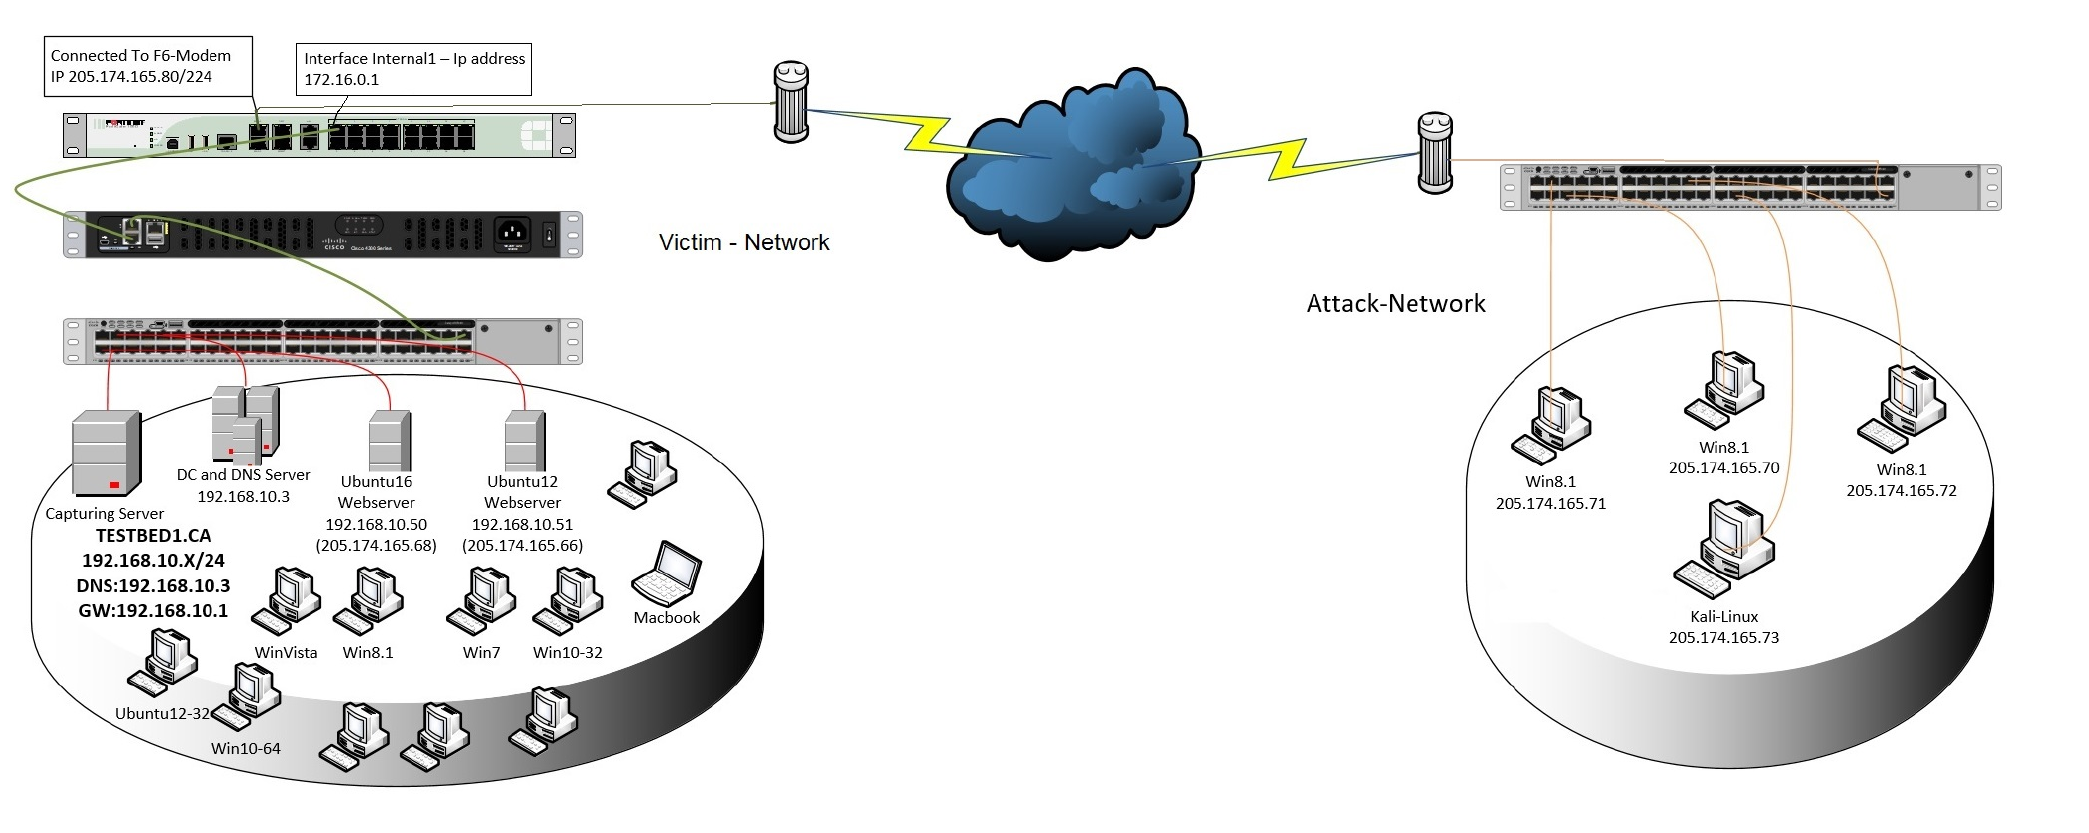
\includegraphics[width=0.9\linewidth]{screenshot001}
	\caption{Architecture of CIC-IDS-2017 testbed}
	\label{fig:cic_2017_testbed}
\end{figure}



\subsubsection{Monday}

On Monday, no attacks take place, only background traffic is happening. The dataset authors utilise a B-Profile system \cite{b_profile} for benign traffic generation "to profile abstract behavior of human interactions and generates naturalistic background traffic"\cite{cic_2017}. The traffic capture of this day consists of "abstract behaviour of 25 users based on the HTTP, HTTPS, FTP, SSH, and email protocols." \cite{cic_2017} and is an excellent source of benign samples that we later use in our experiments.

\subsubsection{Tuesday}
On Tuesday, in addition to the background traffic as seen on Monday, we see the first attack class take place: Bruteforce. In the morning, an FTP Bruteforce attack is performed using Patator \cite{patator}. This attack is run against the iscxtap user, with various passwords being tried from an unknown wordlist. In the afternoon, SSH Bruteforce attack is performed using presumably the same tool. Due to inherent encryption of SSH traffic, it is unclear against which user the attack is conducted or what wordlist is used for passwords.

\subsubsection{Wednesday}
On Wednesday, Denial-of-Service (DoS) attacks are launched against the Ubuntu 16 webserver. The dataset consists of four DoS attacks conducted with the tools Slowhttptest \cite{slowhttptest}, GoldenEye \cite{goldeneye} and HULK \cite{hulk}. In the afternoon, the vulnerable OpenSSH server falls victim to the Heartbleed bug \cite{heartbleed} exploitation.  

Slowhttptest attacks the server by heavily fragmenting the HTTP request body into small chunks and slowly sending them to the server. By slowly receiving the chunks, the server is forced to maintain the connection and waste resources. As the server is limited in how many requests it can serve at any given time, a denial of service occurs.

Slowloris attack works similarly to Slowhttptest, but instead of fragmenting the body, the Headers section of the HTTP request is fragmented. These fragmented headers are then slowly sent to the server, once again forcing it to keep the connection alive and prevent legitimate requests from being processed.

GoldenEye abuses the HTTP \texttt{Connection} and \texttt{Cache-Control} headers to maintain the open connection. Through the \texttt{Connection} HTTP header, the server can be instructed to keep the connection alive (through the \texttt{keep-alive} option) to allow additional requests to take place over the same connection. \texttt{Cache-Control} HTTP header contains instructions for the browser and shared caches. By setting this header to \texttt{no-cache,max-age=0}, it effectively disables connection busting through caches.
GoldenEye abuses these headers by opening a large number of connections, effectively exhausting the connection pool of the server, and denying service to legitimate clients.

Http Unbearable Load King (HULK) attacks the server by flooding it with raw UDP packets. As UDP does not require a three-way handshake to set up a connection like TCP does, this attack can simply flood the server with packets it must handle, overloading it. HULK works best as a distributed attack with multiple malicious clients flooding the target.

The Heartbleed bug \cite{heartbleed} was first discovered in 2014 as a vulnerability in the implementation of the Heartbeat extension proposed by RFC6520. First introduced in December 2011, this bug allows anyone to read the memory of the SSH server due to a missing bounds check \cite{heartbleed_notice}. As the process memory usually contained the unencrypted secret key used to encrypt communications with, it became the primary target of Heartbleed exploits, allowing subsequent decryption of previous and ongoing encrypted communications. CIC-IDS-2017 authors implemented this attack using the Heartleech tool \cite{heartleech} against a vulnerable OpenSSL server version 1.0.1f. 

\subsubsection{Thursday}
On Thursday, authors implement a Web and Infiltration attack classes.

Web attacks consist of attacking the Damn Vulnerable Web App (DVWA) hosted on one the webservers. The authors attack the application by performing a bruteforce attack on the login page of the application and by performing a SQL injection and Cross-Site-Scripting (XSS) attack.

SQL injection attack exploits careless replacements of variables in strings. Malicious strings can alter the behaviour of the query, leaking private information hidden within the database. 

XSS attacks occur when the attacker injects malicious code in to the web application that subsequently gets run for another user. In this instance, SQL injection is performed against the dedicated endpoint for practicing SQL injections provided by DVWA and the XSS attack is conducted by leaking a cookie into the browser's console. 

Infiltration attack is executed by having the user download and execute an infected file on the victim network, which in turn sets up a reverse shell through the Metasploit Framework \cite{metasploit} and allows the attacker to execute portscan of the entire victim network using NMap \cite{nmap}.

\subsubsection{Friday}
On Friday morning, the authors conducted a botnet attack through the Ares \cite{ares} tool, enslaving the computers in the victim network and getting them to take a screenshot of the desktop. 

On Friday afternoon, a Distributed Denial-of-Service (DDoS) attack is conducted against the Ubuntu 16 webserver using the Low Orbit Ion Cannon (LOIC) \cite{loic}. This tool is started on the Windows 8.1 hosts in the attacker network and together, they conduct the DDoS attack.

Finally, last attack class is introduced: Portscan. While we have previously seen this attack as a part the infiltration attack, here we observe it in its raw form. All Windows machines in the victim network are portscanned for running services, using "the main NMap switches such as sS, sT, sF, sX, sN, sP, sV, sU, sO, sA, sW, sR, sL and B." \cite{cic_2017}. In our analysis of the raw PCAP files, we find that switches sF, sX, sP and sA are missing entirely: there is no traffic at the times specified by the dataset authors, nor is there any traffic present that would arise from these switches. Furthermore, the switch -sL performs no attack at all, but simply lists the hosts that would be scanned by the tool. 

\subsubsection{Troubleshooting the dataset}
As alluded to before, Engelen et al. \cite{troubleshooting_cic2017} have performed an extensive analysis of this dataset and found numerous errors in labeling and construction: errors in the construction of the actual flows, imprecise documentation, incorrect labeling, among others. We use their fixed version of the dataset in our experiments.

\subsection{Reconstruction} \label{reconstruction}

As a second step of verifying our hypothesis, we reconstruct the dataset within the ConCap framework. 

ConCap operates on a Kubernetes cluster, spinning up pods that communicate with each other. 
By defining a scenario file in the YAML format, users can easily spin up containers to perform a wide variety of tasks. 
ConCap is designed to capture traffic between pods and analyse it using traffic analysis tools such as CICFlowmeter \cite{cicflowmeter} or Rustiflow \cite{rustiflow}. As ConCap is primarily aimed at constructing attack traffic
In order to construct a scenario, the user can define the attacker and target images, the network configuration and the labelling of generated NetFlows from the traffic occuring on the network. In order to supply the attack tools with the IP addresses of targets, an attack command can be specified with environment variables which will be resolved at runtime.

Having analysed the documentation surrounding the dataset, we notice previously mentioned issues of poor documentation. This leads us to make a number of decisions and guesses in our reconstruction. While we try to remain as faithful as possible to the original dataset, we acknowledge that our implementation may not produce 100\% equivalent network traffic. As our goal is improving the robustness, we focus on reconstructing only the actual attacks and sample the benign traffic from Monday. 

\subsubsection{Tuesday}
In reconstructing the Tuesday attacks, we use Patator by Sebastien Macke \cite{patator}, more specifically its version tagged 0.8. We construct a Docker image containing Patator and a list of usernames and passwords to try against the server. We build this image under the name \texttt{themessik/patator} and push it to Dockerhub. It is unclear what dictionaries authors use for the bruteforce attacks, forcing us to make an arbitrary choice. We choose for a username and password list from the SecLists \cite{seclists} repository: Top Usernames Shortlist\footnote{\url{https://raw.githubusercontent.com/danielmiessler/SecLists/refs/heads/master/Usernames/top-usernames-shortlist.txt}} and Pwdb Top 1000\footnote{\url{https://raw.githubusercontent.com/danielmiessler/SecLists/refs/heads/master/Passwords/Common-Credentials/Pwdb_top-1000.txt}}

\subsubsection{Wednesday}
For the DoS attacks, we use the respective tools mentioned by the dataset authors. We use Sergey Shekyan's Slowhttptest \cite{slowhttptest} tool to reconstruct both Slowhttptest and Slowloris attacks, as this tool provides the required functionality for both. For GoldenEye and HULK, we build dedicated Docker images (\texttt{themessik/goldeneye} and \texttt{themessik/hulk} respectively) and point them at the webserver. For the implementation of the HULK attack, we use a ported version rewritten in Go. This version should maintain the semantics of the original Python tool, as there are multiple such tools named HULK available online, making it unclear which tool the dataset authors use or which one is the original.

For the Heartbleed attack, we build dedicated target image (\texttt{themessik/heartbleed}) based on Ubuntu 16.04 and install the Heartbleed-vulnerable version of OpenSSL 1.0.1f, mirroring the authors. For the attacker image (\texttt{themessik/heartleech}), we use the Robert David Graham's tool heartleech \cite{heartleech} to execute the attack, using the \texttt{--autopwn} option to extract the private key out of the server. 

\subsubsection{Thursday}
On Thursday, we implement the infiltration attack using Damn Vulnerable Web App (DVWA). As we lack access to the authors' specific implementation of this attack, we write our own Python scripts to execute the attacks based on the traffic. For the bruteforce attack, authors seem to use a random string of characters as a password. We opt to make the attack more realistic by using same wordlists as in Tuesday Bruteforce attacks. For the SQL Injection attack, where a lack of input sanitation can expose the entire table, we use the solution provided by the DVWA. For the Cross-Site scripting attack, we inject a \texttt{console.log} statement into the website, similarly to the dataset authors. We package these scripts into a Docker image (\texttt{themessik/dwva\_attacker}) and launch attacks against the official Docker image of DVWA \texttt{vulnerables/web-dvwa}.
	
We choose to omit the Infiltration attacks of Thursday afternoon for two reasons. 
First, we are limited by the ConCap framework. ConCap does not (yet) support multistage attack execution, making it difficult to reproduce this attack faithfully.
Second, and more important, there is little interesting traffic happening on the network in this attack: a file gets downloaded and/or executed and a Portscan is run against the victim network. We will get samples of Portscans on Friday, making the essential repeat of the attack here of little benefit. Furthermore, the maliciousness of a file download is due to the file itself, not the inherent act of downloading a file - this kind of detection is better suited for antivirus software / systems that inspect the files, not network statistics.

\subsubsection{Friday}
On Friday morning, a botnet attack using Ares is executed. We choose to omit this attack in our reconstruction due to technical limitations: Ares does not provide a way to control the botnet from Linux hosts and is reliant on Windows for its execution. Due to this, we cannot package it into a Docker container and execute attacks with it on ConCap.

For Friday afternoon DDoS attack using LOIC, we use the multi-target functionality provided by ConCap. LOIC inherently relies on Windows binaries and its graphical user interface for its function. However, LOIC also provides a way to control it headlessly, through an IRC server. We set up two targets: one the actual webserver we want to attack, the other an IRC server. We have prepared a bot that listens on the IRC channel for LOIC and waits for it to connect. Upon connection, the channel topic is set up as a command for LOIC to attack the webserver. LOIC then proceeds to execute this attack as if it was controlled through the graphical user interface.

Finally, for Portscans, we have analyzed the traffic and enumerated the open ports: 21, 22, 80, 139, 445. These open ports point to following services being online on the server: FTP, SSH, HTTP and SMB. We construct the target Docker image such that all FTP, SSH and HTTP services are available and we execute the attack against this server. SMB has proven exceptionally difficult to get configured this way. We get around this issue by running the Portscan against a dedicated SMB Docker image \texttt{dperson/samba}. This separate traffic later gets merged into other the other Portscan traffic before NetFlows are generated.


	
	\newpage
	\section{Results}
The processed Netflow files can be found on Kaggle. We perform the verification experiment for each attack class separately. 

To quantify the performance of the trained models for different features, we calculate following metrics:

\begin{itemize}
	\item \textbf{Recall}: Recall expresses the correctness of model predictions on positive samples as a ratio of true positives with respect to all positive samples: $$ \frac{TP}{TP+FN} $$
	\item \textbf{Accuracy}: a metric expressing the correctness of predictions of a model as a ratio of the correct predictions and total predictions $$\frac{TP + TN}{TP + TN + FN + FP} $$
	\item \textbf{Precision}: Precision describes how precise the model is in its positive predictions, calcualted as a ratio of true positives and all predicted positives: $$ \frac{TP}{TP+FP} $$
	\item \textbf{Area Under Receiver Operator Characteristic Curve (ROC AUC) score}: By calculating the True Positive Rate and False Positive Rate of the model at set intervals, a curve can be plot through them. Area under this curve expresses how the probability of the model predicting a random malicious sample as malicious. 
	
\end{itemize}

In graphs below, we visualize these metrics for each attack class. Depending on the traffic the model was trained on (Either original CIC-IDS-2017 or ConCap scenarios), we find different sets of features that hold most predictive power. We do note that common features can be found in these sets, and suggest that these features are most representative of the underlying traffic. Consequently, it is these common features that should be used as decision features for actual ML-NIDS systems and we only visualize these features. 

The presence and absence of particular features is a peculiar artifact. We speculate that this can be explained by the difference in the methodology of dataset creation. Our reasons for this are threefold. 

First, though ConCap allows for network features configuration, from bandwidth to packet corruption rate; we have insufficient information about the network conditions of the CIC-IDS-2017 dataset. For this reason, we opt to use the example configuration provided by ConCap authors and keep these conditions the same for all scenarios. 

Second, ConCap networks are built fully in-silico and thus do not suffer from the same artifacts as physical networks might: arbitrary delay in packet processing, faulty connections or interference, as well as processing delay. ConCap network architecture is, without introduction of artificial defects, the perfect network.  

Third, the attacks in the CIC-IDS-2017 dataset take place in addition to benign, background traffic, leading to highly imbalanced datasets. We manually balance the training and testing datasets by including known benign flows to achieve class balance. While this should have little effect on features focusing on the size and content of packets (e.g. Packet Length or Flags features), it will have an effect on features that are more concerned with timings (e.g. Flow Bytes/s or Idle features), as the benign flows had no way of influencing attack flows during traffic capture. 


	
	\newpage
	\section{Conclusion}\label{conclusion}

ML-NIDS systems are the next frontier in NIDS research. Being based on machine learning methods, these systems are capable of learning to distinguish between malicious and benign traffic without the need to manually program them with expert knowledge. These systems do rely on high quality datasets, of which there were numerous attempts to construct and plagued with different issues. 

In this thesis, we have experimentally verified a new method of constructing ML-NIDS datasets through the ConCap framework by reconstructing the CIC-IDS-2017 dataset into ConCap scenarios and showing that the resulting dataset is representative of the original. We find features that hold high predictive power for model training and conclude that ConCap can be used for dataset reconstruction. 

Furthermore, we have further shown that the robustness of ML-NIDS models can be increased by augmenting their training with ConCap traffic, which improves their generalization performance to unseen samples from other datasets. For this, we have generated three variants of attacks already contained in CIC-IDS-2017 and performed adversarial training. Our results show that through adversarial training, ML models can be taught to recognise variants of the attacks without large reductions to their predictive power on the original dataset. 

All of this further cements ConCap (and other such frameworks) as the next step in ML-NIDS dataset generation and augmentation. 
	
	\section{Future Work}\label{future_work}

The road does not end here. While we have verified that ConCap is capable of generating representative traffic, further research is required to build a fully functioning ML-NIDS system around it. Below, we sketch out a number of directions further research could go into.

First, ConCap itself is limited to fully connected networks and simple "run attack command" attacks. In order to be fully representative of our modern networks, support for further network segmentation, switches, firewalls, routers... is needed. In an ideal world, a system administrator should be able to reconstruct their network within ConCap, with all of the fine details that go into configuring a company network. This system administrator should then be able to deploy attacks against the network from a library, train an NIDS system and verify the protections it provides. Furthermore, multi-stage and event-based attacks should be supported, as currently, one cannot easily run a tailored attack based on the current network traffic or conditions.

Second avenue could be a real-time ML-NIDS. The ML model itself is but a small part at the heart of an ML-NIDS system. We have not spent any time studying how to provide the NetFlows to the machine learning model on the fly, instead we post-processed the PCAP files into NetFlows and trained a model on that. While useful, this method will only detect an attack after the fact; and after the fact might be too late, certainly for attacks such as Heartbleed, where leaking the private key spells disaster and could be non-trivial to remediate. A real-time ML-NIDS could detect an attack while it is taking place, enhancing the security of the network that much more.

Third, ConCap can be used not just for its generation capabilities, but also for simulation. This thesis has shown that ConCap is a sound framework for traffic generation, therefore, we propose that this generative capability need not only be used in the context of machine learning, but could also be used as a practical tool for blue team training. Currently, the ConCap environment is spun up, attacks are executed, traffic is captured and the environment is shut down. We envision an environment that remains running, with defenders having the opportunity to train and improve their responses to various attacks.
	
	\section{Extensions}

Here we describe extensions to the attacks we have implemented as part of dataset reconstruction to show the versatility of ConCap as well as the ease of dataset augmentation. 

\subsection{Tuesday attacks}
For Tuesday attacks, we construct the image in such a way that the wordlist used can be easily exchanged for another one. The image \texttt{themessik/patator} does come prepackaged with dictionaries, but these are neither exhaustive nor useful for modelling actual bruteforce attacks. Instead, the attack command can be extended with a flag to download the dictionaries to be used. Instead of specifying the path to the wordlist inside the image, specify a link to download the dictionaries. These will then be downloaded and utilized for attack execution. 

We provide example scenario showing this functionality in \path{scenarios/extensions/tuesday_download_lists.yaml}.
	
	\newpage
	\section{References}
	\printbibliography[heading=none]
	\newpage
	\section{Appendices}
	
	
\end{document}
